%-----------------------------------------------------------------------------
%
%               Template for sigplanconf LaTeX Class
%
% Name:         sigplanconf-template.tex
%
% Purpose:      A template for sigplanconf.cls, which is a LaTeX 2e class
%               file for SIGPLAN conference proceedings.
%
% Guide:        Refer to "Author's Guide to the ACM SIGPLAN Class,"
%               sigplanconf-guide.pdf
%
% Author:       Paul C. Anagnostopoulos
%               Windfall Software
%               978 371-2316
%               paul@windfall.com
%
% Created:      15 February 2005
%
%-----------------------------------------------------------------------------


\documentclass{sigplanconf}

% The following \documentclass options may be useful:

% preprint      Remove this option only once the paper is in final form.
% 10pt          To set in 10-point type instead of 9-point.
% 11pt          To set in 11-point type instead of 9-point.
% numbers       To obtain numeric citation style instead of author/year.

\usepackage[utf8]{inputenc}
\usepackage[T1]{fontenc}
\usepackage{listings}
\usepackage[rgb,dvipsnames]{xcolor}
\usepackage{hyperref}
\usepackage{graphics}
\usepackage{array} % tables
\usepackage{afterpage} % figures
\usepackage{float} % figures
\usepackage{paralist} % figures
\usepackage[shortcuts]{extdash} % figures
\usepackage{todonotes}
\usepackage{textcomp}
\usepackage{ marvosym }
\usepackage{dirtree}
% \usepackage{lmodern}
\usepackage{multirow,tabularx}
\usepackage{ctable}
\usepackage{relsize}
\usepackage{amsmath,amssymb}
\usepackage{algorithm}
\usepackage{algpseudocode}
\usepackage{pifont}
\usepackage{amsthm}
\usepackage{siunitx}
 \sisetup{
    binary-units,
    detect-all,
    free-standing-units,
    space-before-unit,
    use-xspace,
    unit-optional-argument,
    parse-units = false,
  }
%\usepackage[scaled=0.9]{inconsolata}
\usepackage[scaled=0.85]{beramono}
\usepackage[final]{microtype}
\microtypesetup{stretch=9,shrink=15,step=3,letterspace=50}
% % Disable single lines at the start of a paragraph (Schusterjungen)
% \clubpenalty = 10000
% % Disable single lines at the end of a paragraph (Hurenkinder)
% \widowpenalty = 10000 
% \displaywidowpenalty = 10000 % formulas

\usepackage[pass,letterpaper]{geometry}

\usepackage{balance}
%\usepackage{subcaption}
\usepackage{subfig}
\usepackage{wrapfig}

\newcommand{\cL}{{\cal L}}

\lstset{
language=Ruby,
% backgroundcolor=\color[rgb]{0.95, 0.95, 0.95},
tabsize=2,
rulecolor=,
basicstyle=\ttfamily,
upquote=true,
% aboveskip={1.5\baselineskip},
columns=fullflexible,
% columns=fixed,
showstringspaces=false,
extendedchars=true,
breaklines=true,
prebreak = \raisebox{0ex}[0ex][0ex]{\ensuremath{\hookleftarrow}},
% frame=single,
showtabs=false,
showspaces=false,
showstringspaces=false,
% identifierstyle=\ttfamily,
keywordstyle=\color[rgb]{1.0,0,0},
keywordstyle=[1]\color[rgb]{0,0,0.75},
keywordstyle=[2]\color[rgb]{0.5,0.0,0.0},
keywordstyle=[3]\color[rgb]{0.127,0.427,0.514},
keywordstyle=[4]\color[rgb]{0.4,0.4,0.4},
commentstyle=\color[rgb]{0,0,0},
stringstyle=\color[rgb]{0.639,0.082,0.082},
morekeywords={self, proceed},
%numbers=left,%
numbersep=5pt,%
numberstyle=\tiny\color{gray},%
emphstyle=\bfseries,%
breaklines=true,
breakatwhitespace=true,%
escapechar=`,
}
\lstset{escapeinside={<@}{@>}}

\begin{document}

\special{papersize=8.5in,11in}
\setlength{\pdfpageheight}{\paperheight}
\setlength{\pdfpagewidth}{\paperwidth}

\conferenceinfo{ARRAY '16}{Month d--d, 20yy, Malaga, Spain}
\copyrightyear{2016}
\copyrightdata{978-1-nnnn-nnnn-n/yy/mm}
\copyrightdoi{nnnnnnn.nnnnnnn}

% Uncomment the publication rights you want to use.
%\publicationrights{transferred}
\publicationrights{licensed}     % this is the default
%\publicationrights{author-pays}
\toappear{}

\titlebanner{Submitted for review to ARRAY 2016}        % These are ignored unless
\preprintfooter{Layer-based Class Extensions in Squeak/Smalltalk}   % 'preprint' option specified.

\title{Ikra: Object-oriented GPGPU Programming \\ in Ruby with CUDA}
%\title{A Layer-based Approach to Hierarchical Dynamically-scoped Class Extensions}

%\subtitle{Subtitle Text, if any}
\newcommand\Mark[1]{\textsuperscript#1}  
\authorinfo{Matthias Springer\and Hidehiko Masuhara}
           {Department of Mathematical and Computing Sciences, Tokyo Institute of Technology, Japan}
           {matthias.springer@acm.org \and masuhara@acm.org}     
\maketitle

\setcitestyle{square}

\captionsetup{labelfont=bf}

\begin{abstract}

\end{abstract}

\category{D.3.3}{Programming Languages}{Language Constructs and Features}

% general terms are not compulsory anymore,
% you may leave them out
%\terms
%term1, term2

\keywords
Class extension, context-oriented programming, mixins

\section{Introduction}
With the availability and affordability of powerful GPUs, general purpose computing on graphics processing units (GPGPU) is becoming more and more popular in high-performance computing. Nowadays, many supercomputers rely on GPUs as main processing units, because they allow for massively parallel execution of algorithms or simulations with thousands of threads per GPU. However, GPU programming differs from traditional CPU programming, mostly because of architectural differences.

The goal of the Ikra project is to make GPU programming available to researchers who are not familiar with the details of GPUs their programming languages. Ikra is a library for Ruby that translates parallel sections to CUDA code and executes them in parallel on GPUs. We target the Ruby programming language because it provides powerful mechanisms for embedding DSLs in the language, which will be useful for later experiments.

\section{Example: Traffic Simulation}
A simple actor-based traffic simulation will serve as a running example in this paper. The basic idea is to simulate the behavior of a number of actors (e.g., cars, buses, pedestrians, etc.), given a street network as a directed graph (Figure~\ref{fig:running_example}) in adjacency list representation. Every actor is located on one street. Every street has a \emph{length} attribute and every actor has a \emph{progress} attribute representing the distance from the beginning of the street. Once these two attributes have the same value, the actor reached an intersection and should be moved to a different street (or make a U-turn if there is no other neighboring street).

A car moves at a constant speed of \texttt{@max\_velocity}. A predestrian moves at a random speed between $-0.5 \times \texttt{@max\_velocity}$ and $\texttt{@max\_velocity}$, i.e., a pedestrian can make negative progress. This is how we model strolling pedestrains. Furthermore, the progress of actors might be affected by weather conditions depending on their type. For example, cars slow down if the weather conditions are bad, whereas pedestrians are not affected by weather conditions.

\begin{figure}[!htp]
    \centering
    \subfloat[Actual street network (map)]{{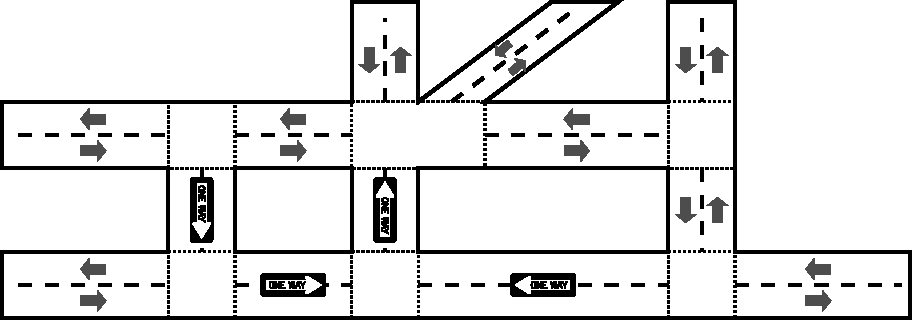
\includegraphics[width=\columnwidth]{running_example.pdf} }}%
    
    \subfloat[Street network as directed graph]{{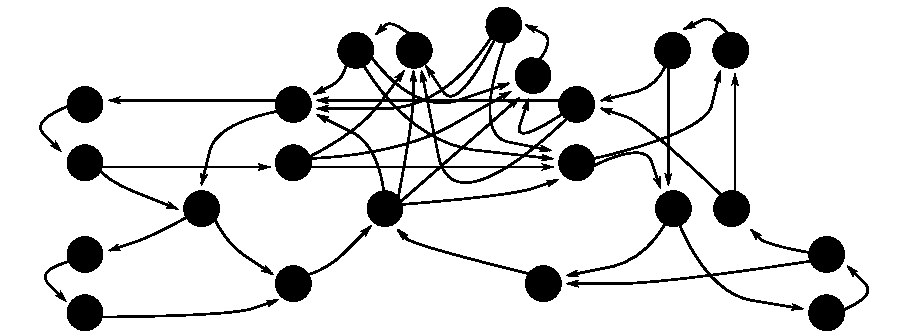
\includegraphics[width=\columnwidth]{running_example_graph.pdf} }}%
    \caption{Street Network for Traffic Simulation}
    \label{fig:running_example}%
\end{figure}

\paragraph{Data Structure}
\begin{figure}[!htp]
    \centering
    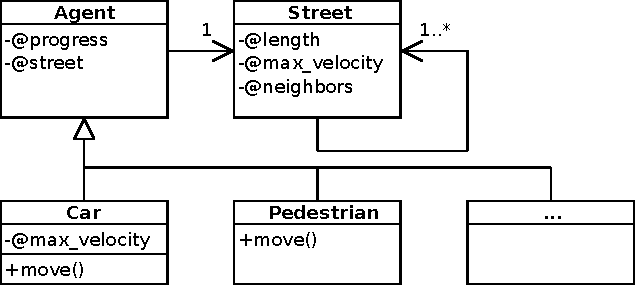
\includegraphics[width=0.8\columnwidth]{class_diagram_running_ex.pdf}
    \caption{Class Diagram for Traffic Simulation}
    \label{fig:running_example_classes}
\end{figure}

The street network and the actors are designed in an object-oriented way. Figure~\ref{fig:running_example_classes} shows the class organization of the traffic simulation. \texttt{Car} and \texttt{Pedestrian} are subclasses of \texttt{Actor} and provide their own \texttt{move} methods which will be invoked for every tick of the simulation. 

\paragraph{Main Simulation Loop}
The following code snippet contains the main simulation functionality. The method \texttt{pmap} designates a parallel section. Its parameter \texttt{ticks} determines how often the entire \texttt{peach} statement should be executed and is equivalent to wrapping the \texttt{peach} statement in a loop that executes it \texttt{ticks} times\footnote{Ikra does not support nested loops properly, which is why we suggest using this shortcut. See Section~\ref{sec:nested_loops} for more details.}.

\begin{lstlisting}
actors = [...]
ticks = 1000
weather = Weather::Rainy

actors.peach(ticks) do |actor|
    actor.move(weather)
end
\end{lstlisting}


\section{Architecture}
Ikra is a library for Ruby. It adds functionality to arrays to execute \texttt{map}, \texttt{select} and \texttt{each} operations in parallel. Programmers can \emph{require} Ikra in Ruby files, upon which new parallel versions of array operations are available (e.g., \texttt{pmap}). These parallel array operations take a block as an argument and designate the only parts of a Ruby programs that are parallelized using Ikra. The default behavior is to spawn one thread per array element, which is why all these computations must be independent of each other. Every \emph{tick} of the simulated progresses the current time by a certain constant value and actors are required to update their progress and street attributes accordingly.

\subsection{Compilation Process}
Figure~\ref{fig:overview_arch} gives a high-level overview of Ikra's compilation process. Upon invocation of a parallel section, Ikra acquires the source code of the parallel block, generates an abstract syntax tree (AST), and infers the type of all expressions. As a result, the type of every local and instance variable is known. In the best case, the type of an expression is monomorphic and primitive, but Ikra also supports arbitrary Ruby classes as types, as well as polymorphic types (see Section~\ref{sec:polymorphic}). The type inferer traverses invoked methods in a may-point-to fashion\footnote{Methods of all possible receiver types are taken into account.}. Based on the type-annotated AST, Ikra generates CUDA kernel code and boilerplate code for kernel invocation, and compiles the CUDA code using the nVidia CUDA toolchain. The result is a shared library which is loaded via Ruby's foreign function interface. Before kernel invocation, the base array along with all reachable objects (via instance variables) is transferred to the GPU's global memory. After kernel invocation, all changed objects and the result of the parallel section (if applicable) are written back to Ruby.

\begin{figure}[!htp]
    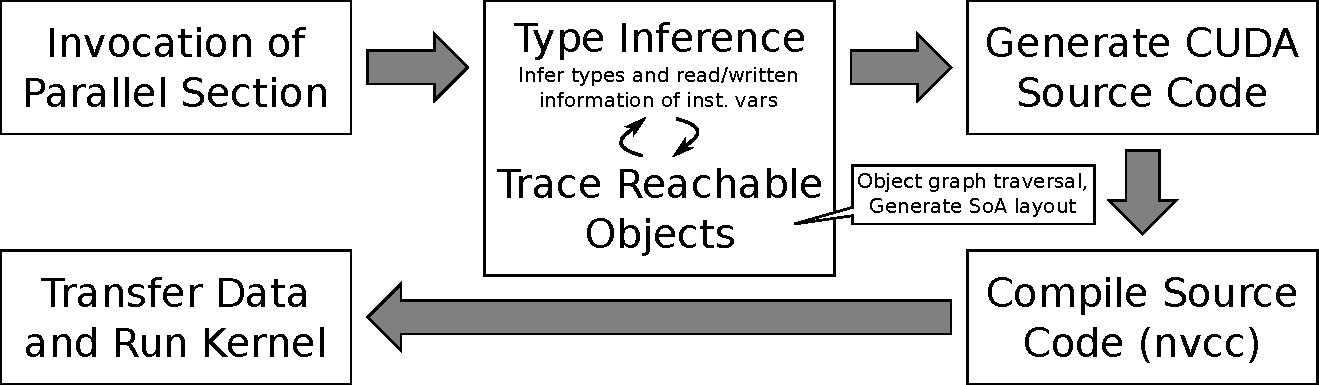
\includegraphics[width=\columnwidth]{high_level_arch.pdf}
    \caption{Overview of Ikra's Architecture}
    \label{fig:overview_arch}
\end{figure}

\subsection{Integration in Ruby}
In contrast to some other projects, Ikra transforms Ruby code to CUDA code while the Ruby program is running (just-in-time compilation). Therefore, Ikra can determine the types of variables that are passed into parallel sections at runtime instead of doing a dataflow analysis of the entire program. This is not only faster but also more accurate in the light of reflection and metaprogramming, which is allowed outside of parallel sections but not inside them.

Two different kinds of variables can be used inside a parallel section: iterator variables and lexical variables. In the following code snippet, \texttt{el} is an iterator variable and \texttt{increment} is a lexical variable. The types of these variables are used as the foundation for type inference of the remaining parallel section.
\begin{lstlisting}
increment = 10
[1, 2, 3].pmap do |el|
    el + increment
end
\end{lstlisting}

Programmers can use not only primitive objects (\texttt{Fixnum}, \texttt{Float}, etc.) but also objects which are instances of Ruby classes inside parallel sections, allowing for object-oriented modelling of the problem (e.g., a traffic simulation). Consequently, a graph of \emph{reachable} (connected) objects must be transferred to the GPU. The \emph{object tracer} is responsible for determining which objects should be copied to the GPU's global memory (see Section~\ref{sec:impl_tracer}).

After kernel execution, changed local variables and instance variables are copied back to the Ruby side (see Section~\ref{sec:impl_copyback}).


\section{Implementation and Optimizations}
In this section, we give an overview of some interesting aspects of Ikra's implementation.

\subsection{Job Reordering}
Before kernel invocation, Ikra analyzes all elements in the base array and reorders them according to their type. This is useful to avoid \emph{thread divergence}, which can penalize performance when running programs on GPUs.

\paragraph{Thread Divergence}
In contrast to most CPU-based systems\footnote{There are CPU extensions for SIMD computations, e.g., SSE.}, GPU-based systems are SIMD (single instruction, multiple data) systems. A GPU consists of a number of streaming multiprocessors. Such a processor has a single control unit that fetches and decodes instructions, but multiple arithmetic logic units (ALUs). Therefore, every instruction is executed in parallel on multiple chunks of data. Every ALU corresponds to one thread, but all threads that are executing on the same stream multiprocessor must follow the same control flow. In case two threads take a different branch, their execution is serialized until the control flow merges again. Consequently, jobs should be threads/jobs should be mapped to streaming multiprocessors in such a way that the control flow is unlikely to divergenge among one such thread group (threads executing on one stream multiprocessor).

In CUDA, such a thread group is called \emph{warp} and typically has a size of 32. There is no explicit interface to allocate threads to warps, but CUDA programmers try to write their programs in such a way that each consecutive group of 32 threads follows the same control flow.

\paragraph{Thread Allocation}
Ikra tries to avoid thread divergence by allocating jobs to warps automatically based on type information. Before kernel invocation, Ikra generates a \emph{job reordering array}, such that the base array is sorted according the elements' types (Figure~\ref{fig:ex_job_reorder}). Ikra does not actually change the order elements in the base array to ensure that other parts of the program outside of the parallel section are not affected.

\begin{figure}[!htp]
    \centering
    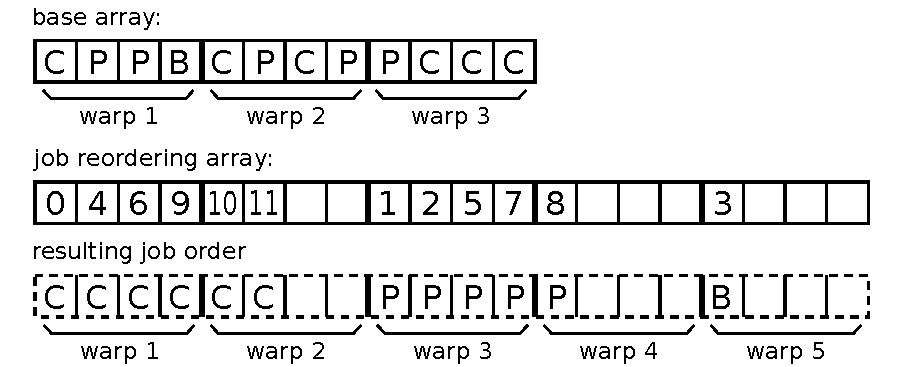
\includegraphics[width=\columnwidth]{reorder_example.pdf}
    \caption{Example: Job Reordering. The first row is the original job order, the second row is the job reordering array, and the third row shows the resulting job order (warp size 4).}
    \label{fig:ex_job_reorder}
\end{figure}

During job reordering the number of threads can increase as shown in Figure~\ref{fig:ex_job_reorder}. Jobs are reordered in such a way that no two elements of different type are allocated in the same warp. If the number of jobs of a particular type is not a multiple of the warp size, the last warp will not be filled up entirely, but some threads will not have a job, i.e., they are not \emph{no operation} threads. This might seem like a waste of computing power, but we expect the number of different types to be small (3 in this example).

The job reordering array can be computed in linear time by scanning all elements of the base array twice. The following pseudo code is similar to counting sort and bucket sort~\cite{Corwin:2004:SLT:1040231.1040257}. It generates one array of indices per type (class) and concatenates these arrays, making sure that every new array starts at a multiple of the warp size $W$.

\begin{algorithm}
\caption{Job Reordering}
\label{CHalgorithm}
\begin{algorithmic}[1]
\Procedure{ReorderingArray}{base, W}
\State $\mathit{types} \gets$ Hash.new
\ForAll {$(\mathit{el}, \mathit{idx}) \in \mathit{base}$}
    \State $\mathit{types}[\mathit{el}.\mbox{class}].\mbox{add}(\mathit{idx})$
\EndFor
\State $\mathit{result} \gets$ Array.new$(\sum_{\mathit{arr} \in \mathit{types}.\mathit{values}} \lceil |\mathit{arr}| / W \rceil * W)$
\State $\mathit{next} \gets 0$
\ForAll {$\mathit{arr} \in \mathit{types}.\mbox{values}$}
    \ForAll {$\mathit{idx} \in \mathit{arr}$}
        \State $\mathit{result}[\mathit{next}] = \mathit{idx}$
        \State $\mathit{next} \gets \mathit{next} + 1$
    \EndFor
    \State $\mathit{next} \gets \lceil \mathit{next} / W \rceil * W$
\EndFor
\State \Return $\mathit{result}$
\EndProcedure
\end{algorithmic}
\end{algorithm}


\subsection{Columnar Object Layout}
Objects are typically represented row-wise, i.e., every object is a contiguous chunk of data in the memory. Based on observations in previous work on GPU-powered database query execution~\cite{Bakkum:2010:ASD:1735688.1735706} where a column-wise data organization proved to be superior compared to a traditional row-based data layout, Ikra stores objects in a columnar layout~\cite{Mattis:2015:COI:2814228.2814230}.

\subsection{Polymorphic Expressions}
\label{sec:polymorphic}
In contrast to CUDA, Ruby is a dynamically-typed programming language. One of the goals of the Ikra project is to allow programmers to write Ruby code in a \emph{natural} way, i.e., without having to think about GPU/CUDA characteristics. For this reason, Ikra should support Ruby expression whose types cannot be inferred unambiguously at translation time.

Ikra embeds dynamic types into CUDA's static type system by generating explicit type dispatch statements at method call sites based on type tags~\cite{Abadi:1989:DTS:75277.75296} for receivers whose types cannot be inferred unambiguously. From a perspective of object-oriented design, this looks as if every object has a \emph{type} instance variable.

\subsection{Read/write Analysis for Instance Variables}

\subsection{Copying back Variables}
\label{sec:impl_copyback}

\subsection{Object Tracer}
\label{sec:impl_tracer}


\section{Optimizations}
% Only write back objects if they are accessed; how can we hook into object access? Proxies?


\section{Benchmarks}

\section{Related Work}

\section{Future Work}

\subsection{Nested Loops}
\label{sec:nested_loops}
Ikra does not yet support nested loops properly. Putting a \texttt{ticks} loop inside the \texttt{peach} block works but contradicts intuition. In a sequential program, most programmers would formulate the simulation code as a series of simulation ticks, where every simulation tick iterates over all actors, as opposed to iterating of over all actors, where every actor is moved for a series of simulation ticks.

\begin{lstlisting}
actors.peach do |actor|
    for i in 1..ticks
        actor.move(weather)
        synchronize
    end
end
\end{lstlisting}

The following code snippet is more intuitive, but would allocate one thread per tick instead of one thread per actor. However, the mechanism described in this paper takes advantage of allocating threads based on the actors' types.
\begin{lstlisting}
(1..ticks).peach do
    actors.each do |actor|
        actor.move(weather)
    end
end
\end{lstlisting}


\section{Conclusion}

% We recommend abbrvnat bibliography style.

\bibliographystyle{plain}
\bibliography{array2016}


\end{document}
